\section{Análise Teórica}

Neste experimento, realizamos a análise teórica de um circuito resistivo
utilizando o método da análise nodal. O objetivo é determinar os potenciais
elétricos nos nós principais, as correntes que circulam pelos resistores e as
potências envolvidas no circuito.

\begin{figure}[H]
  \centering
  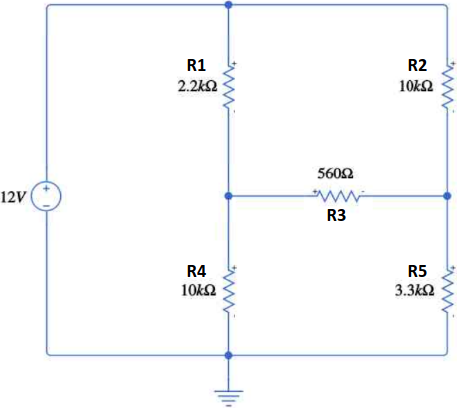
\includegraphics[width=0.5\linewidth]{fig/lab1circuit.png}
  \caption{Circuito para análise em laboratório}
  \label{fig:circuit}
\end{figure}

\subsection{Análise Nodal}

Para determinar as tensões nos nós do circuito, aplicamos a Lei de Kirchhoff das
Correntes (LKC) nos dois principais nós de interesse, denominados \(v_1\) e
\(v_2\). Essa lei estabelece que a soma algébrica das correntes que entram e
saem de um nó é igual a zero.

\begin{itemize}
  \item Nó 1: \(v_1\) (entre R1, R3, R4)
    \[
      \frac{v_1 - 12}{2200} + \frac{v_1 - v_2}{560} + \frac{v_1 - v_2}{10000} = 0
    \]
  \item Nó 2: \(v_2\) (entre R2, R3, R5)
    \[
      \frac{v_2 - 12}{10000} + \frac{v_2 - v_1}{560} + \frac{v_2}{3300} = 0
    \]
\end{itemize}

\subsection{Sistema Linear}

As equações obtidas na análise nodal são reorganizadas para formar um sistema
linear, no qual isolamos os termos relacionados a \(v_1\) e \(v_2\). Isso
facilita a resolução por métodos algébricos.

A seguir, expressamos as equações no formato padrão do sistema:

\[
\left\{
\begin{aligned}
  \left( \frac{1}{2200} + \frac{1}{560} + \frac{1}{10000} \right)v_1 - \left( \frac{1}{560} + \frac{1}{10000} \right)v_2 &= \frac{12}{2200} \\
  - \frac{1}{560}v_1 + \left( \frac{1}{10000} + \frac{1}{560} + \frac{1}{3300} \right)v_2 &= \frac{12}{10000}
\end{aligned}
\right.
\]

Convertendo as frações para valores decimais, obtemos:

\[
\left\{
\begin{aligned}
  0.000988v_1 - 0.001179v_2 &= 0.005455 \\
  -0.001786v_1 + 0.002448v_2 &= 0.0012
\end{aligned}
\right.
\]

Este sistema pode ser resolvido por substituição, método de Gauss ou matriz
inversa. O resultado fornece as tensões nos nós:

\[
  v_1 \approx 7{,}30\,\text{V}, \quad v_2 \approx 6{,}51\,\text{V}
\]

\subsection{Cálculo das Correntes nos Resistores (em mA)}

Com os valores de \(v_1\) e \(v_2\) obtidos, podemos calcular a corrente em cada
resistor usando a Lei de Ohm \(I = \frac{V}{R}\), considerando a queda de tensão
correspondente em cada resistor.

\begin{itemize}
  \item 
    \(I_{R1} = \frac{12 - v_1}{2200} = \frac{4.70}{2200} \approx \SI{2.14}{\milli\ampere}\)
  \item
    \(I_{R2} = \frac{12 - v_2}{10000} = \frac{5.49}{10000} \approx \SI{0.549}{\milli\ampere}\)
  \item
    \(I_{R3} = \frac{v_1 - v_2}{560} = \frac{0.79}{560} \approx \SI{1.41}{\milli\ampere}\)
  \item
    \(I_{R4} = \frac{v_1 - v_2}{10000} = \frac{0.79}{10000} \approx \SI{0.72}{\milli\ampere}\)
  \item
    \(I_{R5} = \frac{v_2 - 0}{3300} = \frac{6.51}{3300} \approx \SI{1.97}{\milli\ampere}\)
\end{itemize}

\subsection{Cálculo das Tensões nos Resistores (em V)}

A tensão sobre cada resistor também pode ser obtida via \(V = R \cdot I\),
confirmando os valores já utilizados no cálculo das correntes.

\begin{itemize}
  \item \(V_{R1} = R_1 \cdot I_{R1} = 2200 \cdot 0.00214 = \SI{4.70}{\volt}\)
  \item \(V_{R2} = 10000 \cdot 0.000549 = \SI{5.49}{\volt}\)
  \item \(V_{R3} = 560 \cdot 0.00141 = \SI{0.79}{\volt}\)
  \item \(V_{R4} = 10000 \cdot 0.000079 = \SI{7.28}{\volt}\)
  \item \(V_{R5} = 3300 \cdot 0.00197 = \SI{6.51}{\volt}\)
\end{itemize}

\subsection{Cálculo da Potência Dissipada por Cada Resistor (em mW)}

A potência dissipada em cada resistor é calculada por \(P = V \cdot I\), sendo
importante para avaliar o consumo energético e a viabilidade dos componentes.

\begin{itemize}
  \item \(P_{R1} = 4.70 \cdot 0.00214 \approx \SI{10.06}{\milli\watt}\)
  \item \(P_{R2} = 5.49 \cdot 0.000549 \approx \SI{3.01}{\milli\watt}\)
  \item \(P_{R3} = 0.79 \cdot 0.00141 \approx \SI{1.11}{\milli\watt}\)
  \item \(P_{R4} = 0.79 \cdot 0.000079 \approx \SI{5.29}{\milli\watt}\)
  \item \(P_{R5} = 6.51 \cdot 0.00197 \approx \SI{12.82}{\milli\watt}\)
\end{itemize}

\subsection{Corrente e Potência da Fonte}

Finalmente, é possível calcular a corrente total fornecida pela fonte somando as
correntes nos ramos diretamente ligados a ela. A potência fornecida é então:

\begin{itemize}
  \item Corrente da fonte: \(I = I_{R1} + I_{R2} = 2.14 + 0.549 = \SI{2.69}{\milli\ampere}\)
  \item Potência fornecida: \(P = V \cdot I = 12 \cdot 0.00269 = \SI{32.28}{\milli\watt}\)
\end{itemize}

Esses resultados permitem validar a consistência do circuito e avaliar se os
componentes estão operando dentro de suas especificações.